\documentclass[review]{elsarticle}

\usepackage{lineno,hyperref}
\modulolinenumbers[5]


% Packages rajoutés par PM
\usepackage{graphicx}
\usepackage{tikz}
\usetikzlibrary[positioning,arrows, arrows.meta]



\journal{Journal of \LaTeX\ Templates}

%%%%%%%%%%%%%%%%%%%%%%%
%% Elsevier bibliography styles
%%%%%%%%%%%%%%%%%%%%%%%
%% To change the style, put a % in front of the second line of the current style and
%% remove the % from the second line of the style you would like to use.
%%%%%%%%%%%%%%%%%%%%%%%

%% Numbered
%\bibliographystyle{model1-num-names}

%% Numbered without titles
%\bibliographystyle{model1a-num-names}

%% Harvard
%\bibliographystyle{model2-names.bst}\biboptions{authoryear}

%% Vancouver numbered
%\usepackage{numcompress}\bibliographystyle{model3-num-names}

%% Vancouver name/year
%\usepackage{numcompress}\bibliographystyle{model4-names}\biboptions{authoryear}

%% APA style
%\bibliographystyle{model5-names}\biboptions{authoryear}

%% AMA style
%\usepackage{numcompress}\bibliographystyle{model6-num-names}

%% `Elsevier LaTeX' style
\bibliographystyle{elsarticle-num}
%%%%%%%%%%%%%%%%%%%%%%%

\begin{document}

\begin{frontmatter}

\title{Un apport de l’IA aux crises épidémiologiques \\ Kiss the Covid}



\author[cristal]{P.~Mathieu\corref{cor1}\fnref{fn1}}
\ead{philippe.mathieu@univ-lille.fr}

\cortext[cor1]{Corresponding author}
\fntext[fn1]{}

\author[cristal]{N.~Mauhé}
\ead{nicolas.mauhe@univ-lille.fr}

\address[cristal]{Univ. Lille, CNRS, Centrale Lille, UMR 9189 --  CRIStAL Lab, F-59000 Lille, France}


\begin{abstract}
  Lors d'une crise sanitaire liée à l'apparition d'une maladie
  infectieuse, il est impératif d'avoir des systèmes d'aide à la
  décision des politiques publiques (évolution de la maladie, immunité
  collective, nombres dates et durées de périodes de
  confinement). \\
  L'évolution d'une maladie infectieuse peut-être modélisée de
  différentes façons (approche centrée-individus, réseaux sociaux,
  equations mathématiques, modèles de flux).\\
  Toutes ces modélisations necessite l'usage de paramètres pour
  calibrer le modèle.\\
  Plus il y a de paramètres, plus il est facile de coller aux
  données (tout comme il existe toujours un polynome de degrès $n$ qui passe par $n$ points).\\
  Certains modélisateurs pensent que plus les paramètres sont précis
  (et nombreux), plus le modèle sera fiable. C'est un course
  sans fin.\\
  L'important est de trouver l'essence du problème, le modèle le plus
  économe en paramètres (parcimonieux) rendant compte des
  phénomènes observés. \\
  L'IA est d'une grande aide pour éviter les biais et régler au mieux
  ces modèles.
\end{abstract}

\begin{keyword}
Infectious disease \sep SIR modelling \sep Decision support system \sep artificial intelligence
\MSC[2010] 00-01\sep  99-00
%http://www.ams.org/msc/msc2010.html
\end{keyword}

\end{frontmatter}

\linenumbers

\section{Introduction (ce qui se fait en épidémio)}

Depuis exactement un siècle et le papier séminal de Kermack et
McKendrick, la modélisation épidémiologique a pris une part
prépondérante dans l’étude de ces phénomènes complexes. La crise du
H1N1 en 2008 a nettement amplifié ce phénomène, faisant apparaître un
nombre important de modèle tous plus complexe les uns que les
autres. Dans ce papiers nous montrons que les techniques
d’intelligence artificielle Utilisées à bon escient, Permettent d’une
part de concevoir des modèles plus facile à comprendre et à utiliser
par les thématiciens et d’autre part de faciliter grandement la
conception d’outils d’aide à la décision pour les politiques
sanitaires.


Le modèle présenté s'appuie sur des taux de contagion
adaptable chaque jour, dont la valeur est automatiquement calculée par
apprentissage génétique.



Le modèle SIR de Kermack et McKendrick \cite{} a été proposé en 1927 pour expliquer la hausse et la baisse rapides du nombre de patients infectés observées lors d'epidémies telles que la peste (à Londres en 1665, à Bombay en 1906) ou le choléra (à Londres en 1865). Il a été remis à l’avant-plan à la fin des années 1970 par Anderson et May \cite{}.


\bigskip


\hfill \scalebox{.75}{
	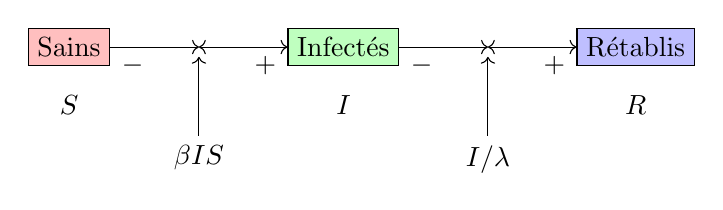
\begin{tikzpicture}[node distance=1cm,
          boite/.style={draw,rectangle, minimum width=1cm, fill=#1!25}]
          \node[boite=red](leftNode) {Sains};
	        \node[below=0.25cm of leftNode](labelLeftNode) {\(S\)};
		\node[right=of leftNode](middleLeft) {};
		\node[boite=green,right=of middleLeft](centralNode) {Infectés};
		\node[below=0.25cm of centralNode](labelCentralNode) {\(I\)};
		\node[right=of centralNode](middleRight) {};
		\node[boite=blue,right=of middleRight](rightNode) {Rétablis};
		\node[below=0.25cm of rightNode](labelRightNode) {\(R\)};
		\draw[->] (leftNode) --node[below, near start]{\(-\)} (middleLeft.center);
		\draw[<->] (middleLeft.center) --node[below, near end]{\(+\)} (centralNode);
		\draw[->] (centralNode) --node[below, near start]{\(-\)} (middleRight.center);
		\draw[<->] (middleRight.center) --node[below, near end]{\(+\)} (rightNode);
		\node[below=of middleLeft](leftLabel){\(\beta I S\)};
		\node[below=of middleRight](rightLabel){\(I / \lambda\)};
		\draw[->] (leftLabel) -- (middleLeft);
		\draw[->] (rightLabel) -- (middleRight);
	\end{tikzpicture}
} \hfill \



\section{L'apport de l'informatique}

L'usage de l'IA est une méthode nouvelle pour l'épidémio, mais ancienne pour l'informatique.


Certains pensent que si on complexifie le modèle, on s'approche de la réalité : or plus il y a de paramètres, plus c'est facile de ``fitter'' : Problématique de l'overfitting (mettre une belle courbe qui passe par n points alors qu'en fait c'est une droite qui généralise le mieux).


\begin{figure}[h]
  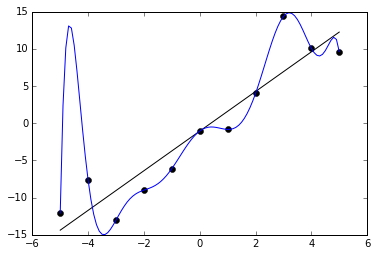
\includegraphics[width=0.8\linewidth]{Overfitted_Data.png}  
  \centering
  \caption{\copyright \href{wikipedia}{https://en.wikipedia.org/wiki/Overfitting}  Des données bruitées (approximativement linéaires) sont approximées par une fonction linéaire et une fonction polynomiale. Bien que la fonction polynomiale soit parfaitement ajustée, on constate que la fonction linéaire généralise surement bien mieux}
  \label{fig:overfitting}
\end{figure}


Un modèle qui ne fonctionne pas (parce que par exemple des R0 sont délirants) peut très bien néanmoins ``fitter'' les données  et donc continuer à prédire correctement les personnes en Réa


L'apport de l'informatique :
\begin{itemize}
\item des techniques et des outils : algos d'apprentissage
\item s'attacher à l'essence du problème : principe de parcimonie
\end{itemize}


\section{Hypothèse de simplicité}

Avce quelque chose de très simple on ``fitte'' les données

\bigskip

\hfill \scalebox{.75}{
	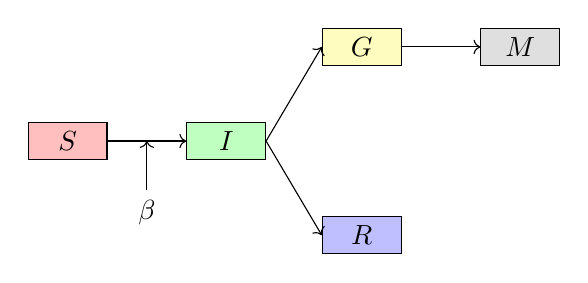
\begin{tikzpicture}[node distance=1cm,
		boite/.style={draw,rectangle, minimum width=1cm, fill=#1!25}]
		\node[boite=red](premier){\(S\)};
		\node[boite=green, right=of premier](second){\(I\)};
		\draw[->] (premier) -- node[midway](milieu){} (second);
		\node[below=.5cm of milieu](labelMilieu){\(\beta\)};
		\draw[->] (labelMilieu) -- (milieu.center);
		\node[boite=yellow, above right=of second](troisHaut){\(G\)};
		\draw[->] (second.east) -- (troisHaut.west);
		\node[boite=blue, below right=of second](troisBas){\(R\)};
		\draw[->] (second.east) -- (troisBas.west);
		\node[boite=gray, right=of troisHaut](quatre){\(M\)};
		\draw[->] (troisHaut) -- (quatre);
	\end{tikzpicture}
} \hfill \

\bigskip

\hfill \scalebox{.75}{
	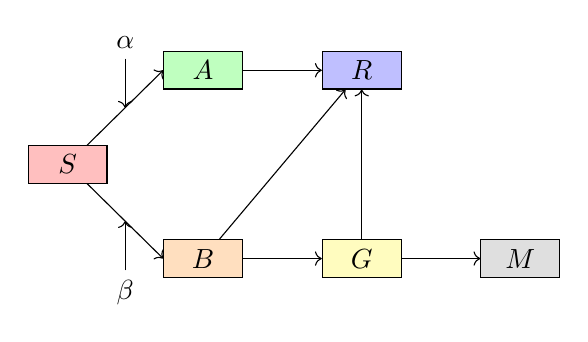
\begin{tikzpicture}[node distance=1cm,
		boite/.style={draw,rectangle, minimum width=1cm, fill=#1!25}]
		\node[boite=red](premier){\(S\)};
		\node[boite=green, above right=of premier](secondHaut){\(A\)};
		\draw[->] (premier) -- node[midway](milieuHaut){} (secondHaut.west);
		\node[above=.5cm of milieuHaut](labelMilieuHaut){\(\alpha\)};
		\draw[->] (labelMilieuHaut) -- (milieuHaut.center);
		\node[boite=orange, below right=of premier](secondBas){\(B\)};
		\draw[->] (premier) -- node[midway](milieuBas){} (secondBas.west);
		\node[below=.5cm of milieuBas](labelMilieuBas){\(\beta\)};
		\draw[->] (labelMilieuBas) -- (milieuBas.center);
		\node[boite=blue, right=of secondHaut](troisHaut){\(R\)};
		\draw[->] (secondHaut) -- (troisHaut);
		\draw[->] (secondBas) -- (troisHaut);
		\node[boite=yellow, right=of secondBas](troisBas){\(G\)};
		\draw[->] (secondBas) -- (troisBas);
		\draw[->] (troisBas) -- (troisHaut);
		\node[boite=gray, right=of troisBas](quatre){\(M\)};
		\draw[->] (troisBas) -- (quatre);
	\end{tikzpicture}
} \hfill \



\begin{center}
  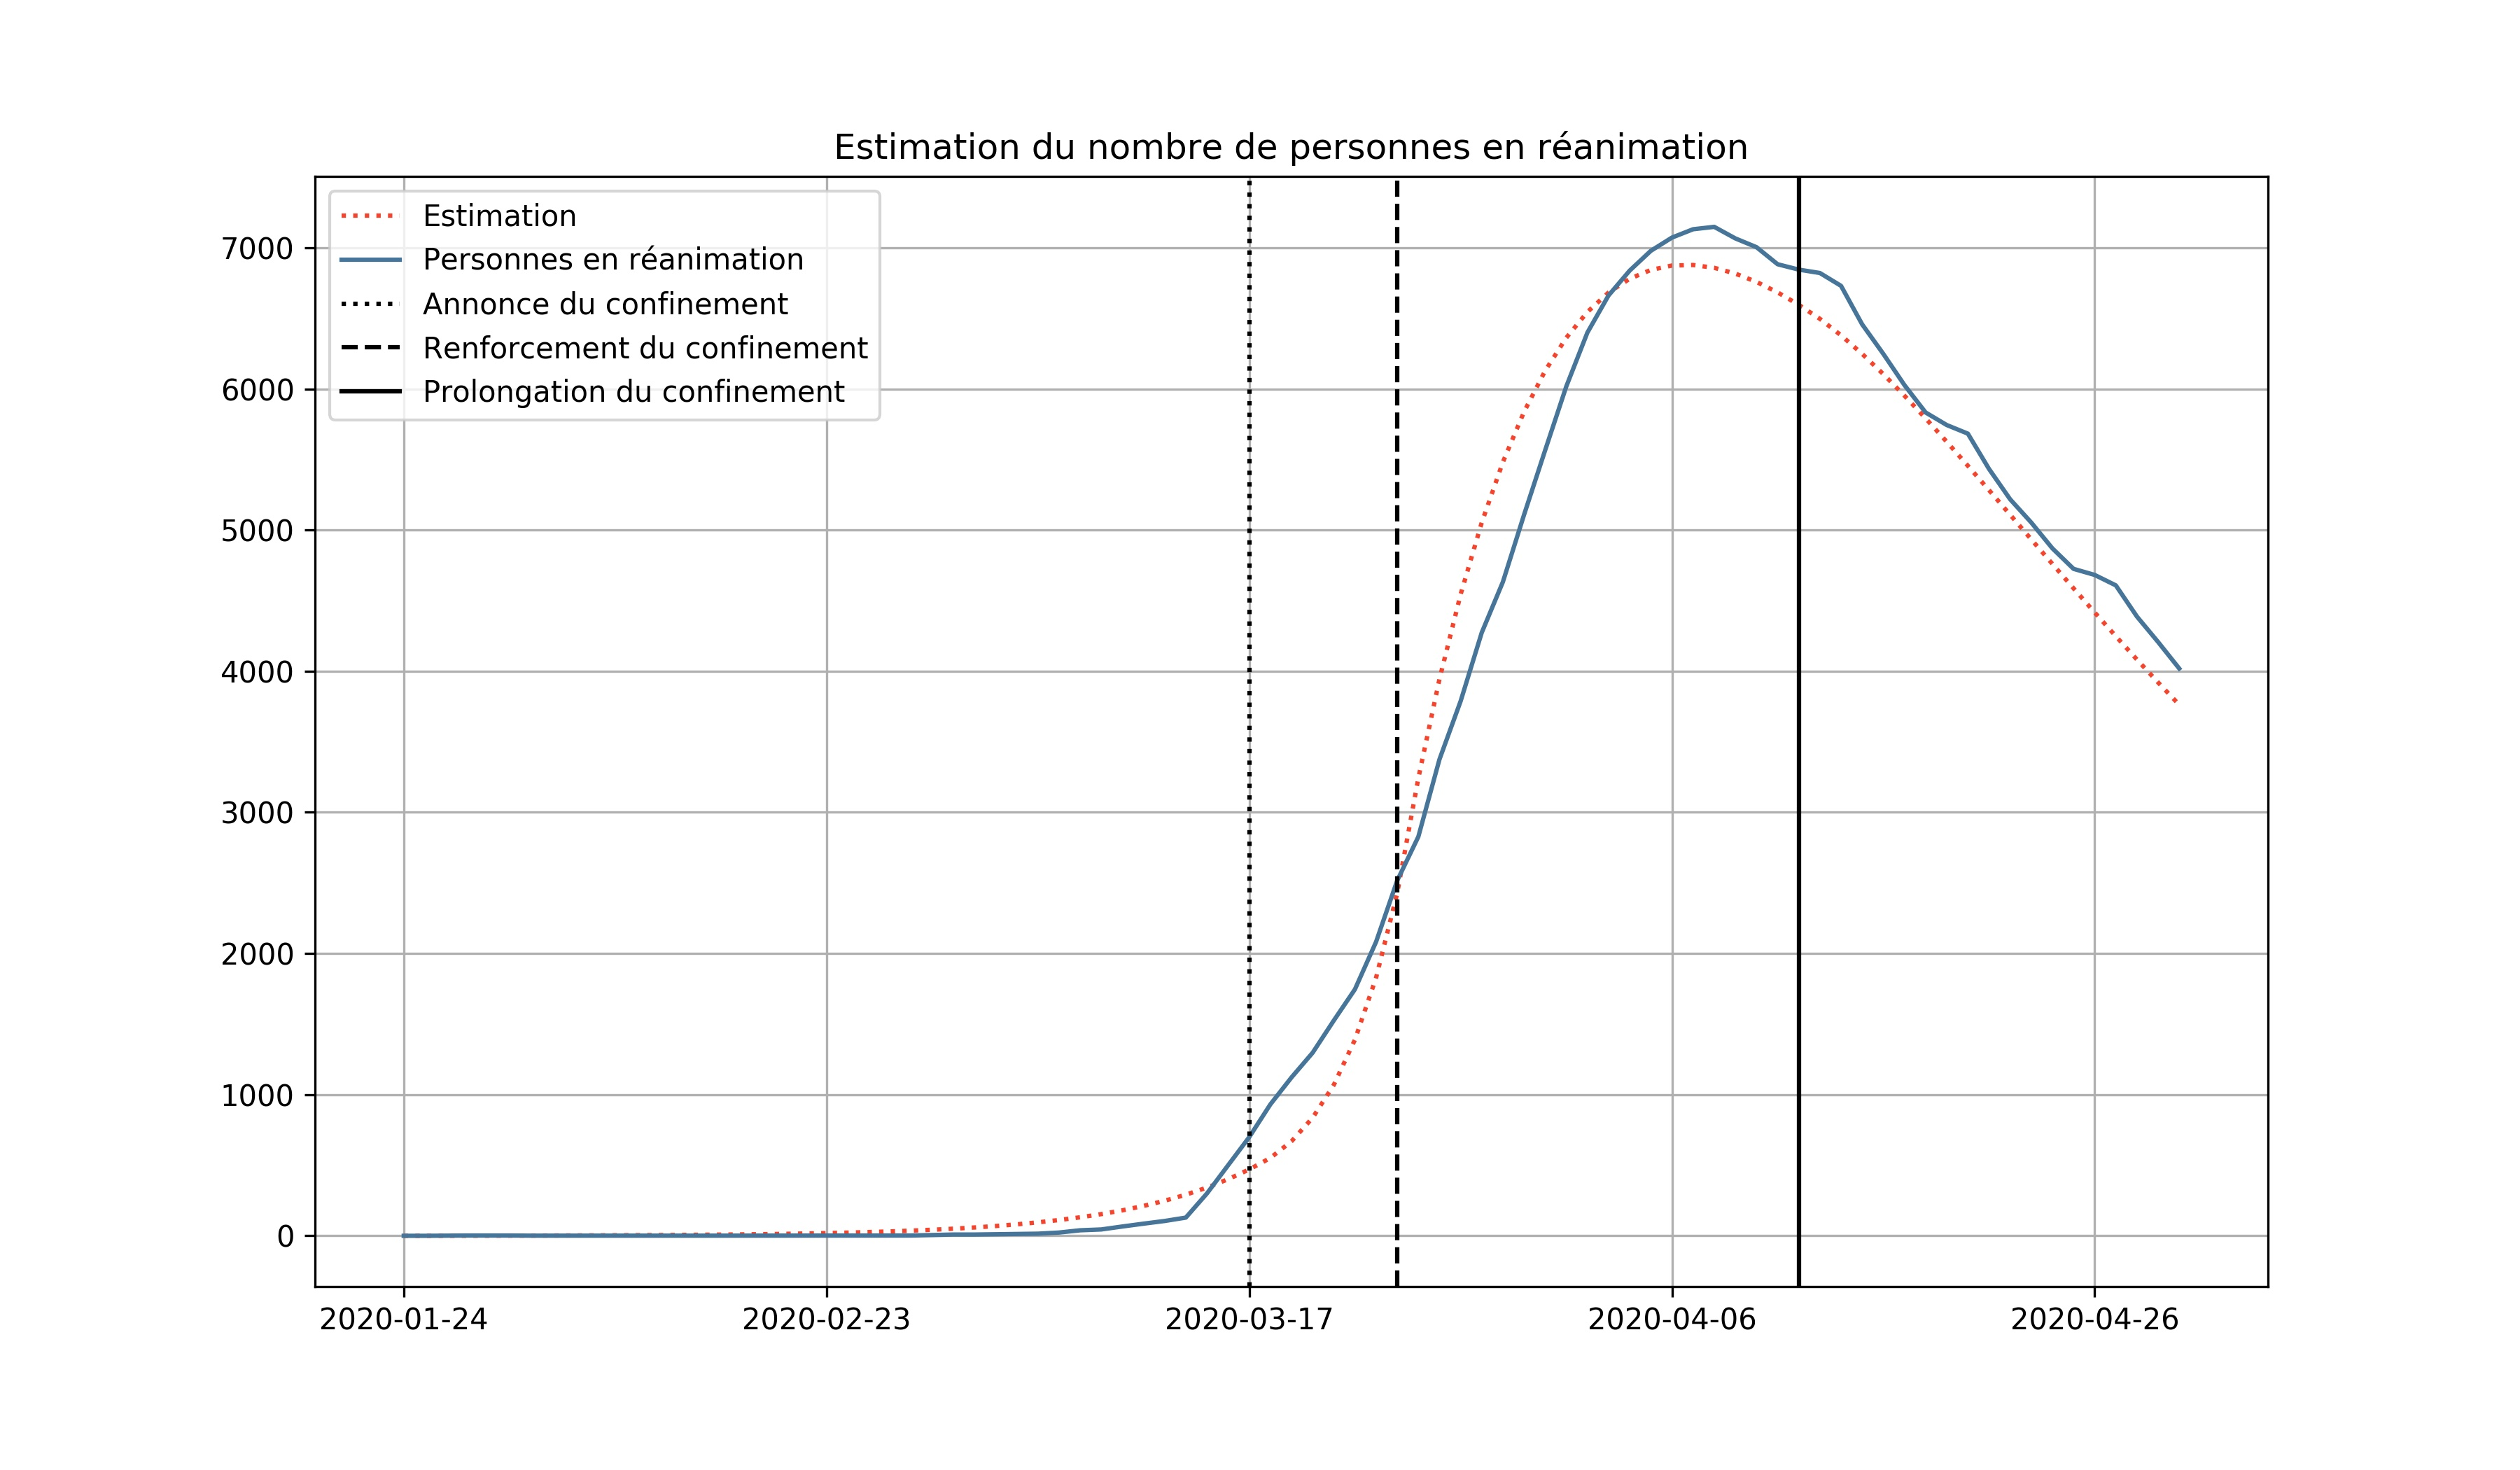
\includegraphics[width=0.8\linewidth]{../slides/figure1.jpg}
\end{center}

\section*{References}

\bibliography{kiss_covid}
\nocite{*}

\end{document}